\documentclass[a4paper,norsk]{report}
\usepackage[latin1]{inputenc}
\usepackage[T1]{fontenc}
\usepackage{babel}
\usepackage{textcomp,listings, subfigure,graphicx}
\usepackage{subfig}
\setlength\parindent{0pt}
\usepackage{parskip}
\usepackage{listings}
\usepackage{amsmath}
\title{Benchmark}
\author{Sebastian Gjertsen}
\begin{document}
\maketitle

\section*{Fluid Structure Interaction Problem formulation in ALE coordinates}
\subsection*{Introduction}
Here we will look at the ALE formulation of solving the FSI problem. The ALE approach stands for Arbitrary Lagrangian Eulerian, meaning that we define the fluid problem in an Eulerian framework and the solid problem in an Lagrangian framework. The ALE method can be solved by moving the mesh for each time step, following the structure body movements [Houston paperet]. This approach gives advantages as we can explicitly represent the fluid-structure interface. But problems arise when there are large deformations in solid structure, giving major mesh deformations in the fluid mesh. Another way of approaching the ALE-FSI problem is to used reference or fixed meshes. Instead of updating the mesh for each time step, we instead use a series of mappings to map the solution from a reference mesh and onto our current mesh. First we look at the mapping and identities needed to solve the reference approach to ALE.
\subsection*{Reference domain}
\subsection*{Mapping and identites}
\includegraphics[scale=0.4]{continuum_mapping.png}

To get an ALE formulation from a reference frame, we need to define a mapping in the solid domain:
$$  \chi^s(t) : \hat{\mathcal{S}} \rightarrow \mathcal{S}(t)     $$ 
We define the $ \hat{\mathcal{S}}$ as the initial stress free configuration, the $\mathcal{S}$ as the reference and the $\mathcal{S}(t)$ as the current configuration.
The same is for the fluid domain.
$$  \chi^f(t) : \hat{\mathcal{F}} \rightarrow \mathcal{F}(t)     $$ 
The solid mapping is set as $\chi^s(\textbf{X},t) = \textbf{X}  + d^s(\textbf{X} ,t)$
hence giving:
$$  d^s(\textbf{X},t) = \chi^s(\textbf{X},t) -\textbf{X}   $$
$$  w(\textbf{X},t) = \frac{\partial \chi^s(\textbf{X},t)}{\partial t}   $$

where $\textbf{X}$ denote a material point in the reference domain and $\chi^s$ denotes the mapping from the reference configuration.
We denote $\Gamma^1$ as the "ceiling" and "floor" and the circle and $\Gamma^{2,3}$ as the inlet and outlet.
The velocity in the fluid is denoted $u(\textbf{X},t)$
We define the deformation gradient $F = I + \nabla d$ and $J = det(F)$
\subsection*{Balance laws}
We will formulate the equations in the Eulerian, Lagrangian and the ALE description.
The Eulerian description suits a fluid problem nicely as the points in the grid are fixed and the fluid particles move through the domain. Whilst the Lagrangian description fits a solid problem as the material particles are fixed with the gridpoints. The fluid velocity vector and the displacement vector are the quantities describing motion of the fluid and solid respectively. Since we here have fluid structure interaction problem we need to formulate the fluid in the fixed mesh description. The fluid velocity will still be the quantity describing motion but it will also have the displacement of the fluid, describing the change in fluid domain. The solid will be described in Lagrangian. We will only look at incompressible fluids where the volume of the fluid domain stays constant.\\
We express the solid balance laws in the Lagrangian formulation from the initial configuration
$$J\rho_s \frac{\partial^2 d}{\partial t^2} = \nabla \cdot (J \sigma_s F^{-T}) \hspace{4mm}in\hspace{4mm} \mathcal{\hat{S}} $$
Piola-Kirchhoff tensor:
\begin{align*}
 \sigma_s =& \frac{1}{J} F (\lambda_s (tr E)I + 2\mu_s E) F^{-T}  \\
 S_s =& \lambda_s (tr E)I + 2\mu_s E  
\end{align*}
$\lambda_s = \frac{2\mu_s nu_s}{1-2 \nu_s} $, $ E = \frac{1}{2} (F^{T}F -I)$


The fluid equations are denoted from the initial configuration:
$$ \rho_f J \big( \frac{\partial u}{\partial t} + (\nabla u)F^{-1}(u-w)\big) = \nabla \cdot (J\sigma_f F^{-T} )\hspace{4mm} in \mathcal{\hat{F}}$$
$$ \nabla \cdot (J u F^{-T}) = 0 \hspace{4mm} in \hspace{2mm} \mathcal{\hat{F}}$$

To bind together the computation of fluid and structure domain, we need a harmonic extension to the boundary values. For this purpose define the following equation with the fluid domain deformation:
$$ \nabla^2 d^f = 0\hspace{4mm}in \hspace{2mm} \mathcal{\hat{F}}$$
This equation is chosen for its good regularity and smoothing properties.

Boundary conditions:

In the place where the fluid and structure domains meet, i.e the interface. We set a dynamic condition saying that the normal stresses of the solid and fluid are equal:
$$  \sigma_f n_f = \sigma_s n_s \hspace{4mm} on  \hspace{2mm}\Gamma^0 (interface)   $$
These will be written in the Lagrangian formulation:
$$  J\sigma_f F^{-T} n_f = \sigma_s  n_s \hspace{4mm} on  \hspace{2mm}\Gamma^0 (interface)   $$

\subsection*{Domain move}
Here we will look at the approach involving moving the mesh each time step. \\
The fluid equation is simply Navier-Stokes with a domain mapping in the transport term giving:
$$ \rho_f \big( \frac{\partial u}{\partial t} + (\nabla u)(u-w)\big) = \nabla \cdot \sigma_f \hspace{4mm} in \mathcal{F}$$
$$ \nabla \cdot u = 0  \hspace{4mm} in \hspace{4mm} \mathcal{F} $$
After each timestep we update the mesh and compute this equation over the current mesh. The real velocity of the fluid particles is there for the fluid velocity itself minus the velocity of the mesh. 

The solid equations will be formulated similar to before but we can write them with the displacement velocity: $ \frac{\partial d}{\partial t} = u_f $:
$$ \rho_s \frac{\partial u_f}{\partial t} = \nabla \cdot \sigma_s \hspace{4mm}in\hspace{4mm} \mathcal{\hat{S}} $$
Laplace operator:
$$ \nabla^2 d_f = 0\hspace{4mm}in \hspace{2mm} \mathcal{\hat{F}}$$

Boundary conditions stay the same but without mappings:
$$ u = u0 \hspace{4mm}on \hspace{2mm} \Gamma^2$$
We set no slip on the "floor" and "ceiling" so to speak:
$$ u = 0  \hspace{4mm}on \hspace{2mm} \Gamma^1  $$
$$  \sigma_f n_f = \sigma_s n_s \hspace{4mm} on  \hspace{2mm}\Gamma^0 (interface)   $$

The two approaches to the ALE method is equivalent [Godboka]. 
From a technical point of view, both formulations are equivalent. Wether we use a fixed and reference formulation or a moving mesh and Eulerian formulation. 
\subsection*{Variational formulation}
We start by looking at the variational formulation for the reference domain.
We use 3 testfunctions, $\phi, \psi, \gamma$.
\begin{align*}
\rho_f J \big( \frac{\partial u}{\partial t} + (\nabla u)F^{-1}(u-\frac{\partial d}{\partial t}) , \phi\big)_{\mathcal{\hat{F}}} + (J\sigma_f F^{-T},\nabla \phi )_{\mathcal{\hat{F}}} &= 0  \\
 \big( \nabla \cdot (J u F^{-T}),\gamma \big)_{\mathcal{\hat{F}}} &= 0 \\
\big(J\rho_s \frac{\partial u}{\partial t},\phi \big)_{\mathcal{\hat{S}}} + \big(F \sigma_s(d), \nabla \phi \big)_{\mathcal{\hat{S}}} &=0 \\
 \big( \nabla d , \nabla \psi \big)_{\mathcal{\hat{F}}} &= 0 \\
 \big( u- \frac{\partial d}{\partial t} ,\psi \big)_{\mathcal{\hat{S}}} &= 0 \\
\end{align*}

We then look at the variational formulation for moving the mesh, here we employ a global function for u in the fluid and solid. Which is the fluid velocity in the fluid domain and displacement velocity solid domain. And in the last equation we force $w$ to be the solid displacement in the solid domain.
\begin{align*}
\rho_f \big( \frac{\partial u}{\partial t} + (\nabla u)(u-w) , \phi\big)_{\mathcal{F}} + (\sigma_f ,\nabla \phi )_{\mathcal{F}} &= 0  \\
 \big( \nabla \cdot (u ),\gamma \big)_{\mathcal{F}} &= 0 \\
\big(\rho_s \frac{\partial u}{\partial t},\phi \big)_{\mathcal{S}} + \big( \sigma_s(d), \nabla \phi \big)_{\mathcal{S}} &=0 \\
 \big( \nabla d , \nabla \epsilon \big)_{\mathcal{F}} &= 0 \\
 \big( w- u,\epsilon \big)_{\mathcal{S}} &= 0 \\
\end{align*}



\newpage

\section*{Problem Defintion}
\subsection*{Domain}
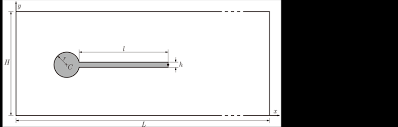
\includegraphics[scale=0.9]{geometry.png}
The computational domain resembles the classic cfd benchmark with an added bar, with dimensions:
The box: L = 2.5, H = 0.41
The bar: l = 0.35, h = 0.02
The circle is positioned at (0.2, 0.2) making it 0.05 of center from bottom to top, this is done to induce oscillations to an otherwise laminar flow.\\
Boundary conditions:\\
The fluid velocity has a parabolic profile on the inlet that changes over time:\\
$$ u(0,y) = 1.5u_0 \frac{y(H-y)}{(\frac{H}{2})^2}  $$
$$ u(0,y,t) = u(0,y)\frac{1-cos(\frac{\pi}{2}t)}{2} \text{  for  } t<2.0$$
$$ u(0,y,t) = u(0,y) \text{  for  } t \leq 2.0 $$

We set no slip on the "floor" and "ceiling" so to speak.\\
On the fluid solid interface the boundary conditions are set to:
$$  \sigma_f n_f = \sigma_s n_s \hspace{4mm} on  \hspace{2mm}\Gamma^0 (interface)   $$
In our variational form we leave this out and so implying that they are equal.


\subsection*{FSI test}
\begin{table}[h]
\centering
\caption{My caption}
\label{my-label}
\begin{tabular}{|l|l|l|l|}
\hline
Parameters & FSI1 & FSI2 & FSI3 \\ \hline
$\rho_f[10^3 \frac{kg}{m^3}]$ & 1 & 1 & 1 \\ \hline
$\nu_f [10^{-3} \frac{m^2}{s}]$ & 1 & 1 & 1 \\ \hline
$u_0$ & 0.2 & 1 & 2 \\ \hline
Re = $\frac{U d}{\nu_f}$ & 20 & 100 & 200 \\ \hline
$\rho_s[10^3 \frac{kg}{m^3}]$ & 1 & 10 & 1 \\ \hline
$\nu_s$ & 0.4 & 0.4 & 0.4 \\ \hline
$\mu_s[10^6 \frac{m^2}{s}]$ & 0.5 & 0.5 & 2 \\ \hline
\end{tabular}
\end{table}








\bibliographystyle{plain}
@article{quaini2014extended,
  title={An extended ALE method for fluid-structure interaction problems with large structural displacements},
  author={Quaini S ?Canic, S Basting A and Glowinski, R},
  year={2014}
}
\bibliography{./Cite/cites}

\end{document}
